
\documentclass[12pt]{article}

% Layout.
\usepackage[top=1in, bottom=0.75in, left=1in, right=1in, headheight=1in, headsep=6pt]{geometry}

% Fonts.
\usepackage{mathptmx}
\usepackage[scaled=0.86]{helvet}
\renewcommand{\emph}[1]{\textsf{\textbf{#1}}}

% TiKZ.
\usepackage{tikz, pgfplots}
\usetikzlibrary{calc}
\pgfplotsset{compat = newest}
 
\pgfplotsset{my style/.append style={axis x line=middle, axis y line=
middle, xlabel={$x$}, ylabel={$y$}, axis equal
}}

% Misc packages.
\usepackage{amsmath,amssymb,latexsym}
\usepackage{graphicx}
\usepackage{array}
\usepackage{xcolor}
\usepackage{multicol}

% Commands to set various header/footer components.
\makeatletter
\def\doctitle#1{\gdef\@doctitle{#1}}
\doctitle{Use {\tt\textbackslash doctitle\{MY LABEL\}}.}
\def\docdate#1{\gdef\@docdate{#1}}
\docdate{Use {\tt\textbackslash docdate\{MY DATE\}}.}
\def\doccourse#1{\gdef\@doccourse{#1}}
\let\@doccourse\@empty
\def\docscoring#1{\gdef\@docscoring{#1}}
\let\@docscoring\@empty
\def\docversion#1{\gdef\@docversion{#1}}
\let\@docversion\@empty
\makeatother

% Headers and footers layout.
\makeatletter
\usepackage{fancyhdr}
\pagestyle{fancy}
\fancyhf{} % Clears all headers/footers.
\lhead{\baselineskip 30pt
%\emph{\@doctitle\hfill\@docdate}
\emph{\@docdate\hfill\@doctitle}
\ifnum \value{page} > 1\relax\else\\
\emph{Name: \rule{3.5in}{1pt}\hfill \@docscoring}\fi}
\rfoot{\emph{\@docversion}}
\lfoot{\emph{\@doccourse}}
\cfoot{\emph{\thepage}}
\renewcommand{\headrulewidth}{0pt}%
\makeatother

% Paragraph spacing
\parindent 0pt
\parskip 6pt plus 1pt

% A problem is a section-like command. Use \problem{5} to
% start a problem worth 5 points.
\newcounter{probcount}
\newcounter{subprobcount}
\setcounter{probcount}{0}
\newcommand{\problem}[1]{%
\par
\addvspace{4pt}%
\setcounter{subprobcount}{0}%
\stepcounter{probcount}%
\makebox[0pt][r]{\emph{\arabic{probcount}.}\hskip1ex}\emph{[#1 points]}\hskip1ex}
\newcommand{\thesubproblem}{\emph{\alph{subprobcount}.}}

% Subproblems are an enumerate-like environment with a consistent
% numbering scheme. 
% Use \begin{subproblems}\item...\item...\end{subproblems}
\newenvironment{subproblems}{%
\begin{enumerate}%
\setcounter{enumi}{\value{subprobcount}}%
\renewcommand{\theenumi}{\emph{\alph{enumi}}}}%
{\setcounter{subprobcount}{\value{enumi}}\end{enumerate}}

% Blanks for answers in normal and math mode.
\newcommand{\blank}[1]{\rule{#1}{0.75pt}}
\newcommand{\mblank}[1]{\underline{\hspace{#1}}}
\def\emptybox(#1,#2){\framebox{\parbox[c][#2]{#1}{\rule{0pt}{0pt}}}}

% Misc.
\renewcommand{\d}{\displaystyle}
\newcommand{\ds}{\displaystyle}
\def\bc{\begin{center}}
\def\ec{\end{center}}
\def\be{\begin{enumerate}}
\def\ee{\end{enumerate}}


\doctitle{Math 251: Quiz 8}
\docdate{Nov 3, 2022}
\doccourse{UAF Calculus I}
\docversion{v-1}
\docscoring{\blank{0.8in} / 25}
\begin{document}

There are 25 points possible on this quiz. No aids (book, calculator, etc.)
are permitted.  {\bf Show all work for full credit.}

\problem{8} Answer the questions below about the function $f(x)=4x^3-3x^4.$ Observe that \\$f'(x)=-12(x-1)x^2$ and $f''(x)=12x(2-3x).$
\begin{subproblems}
	\item Find intervals where $f$ is increasing or decreasing.
	\vfill
	\item  Find $x$-values of any local minima and local maxima of $f$ or state that none exist
	\vfill
	\item  Find intervals where $f$ is concave up and concave down.
	\vfill
	\item  Find $x$-values of any inflection points of $f.$
	\vfill
\end{subproblems}
\problem{3} Find any horizontal asymptotes of the graph $H(x)=5+\frac{x}{2x+1}.$ Show your work.
\vfill
\newpage
\problem{6} Based on the graph of the function $g(x)$ (below) to determine whether each value below is \emph{positive}, \emph{negative}, \emph{zero}, or \emph{undefined}.
\begin{multicols}{2}
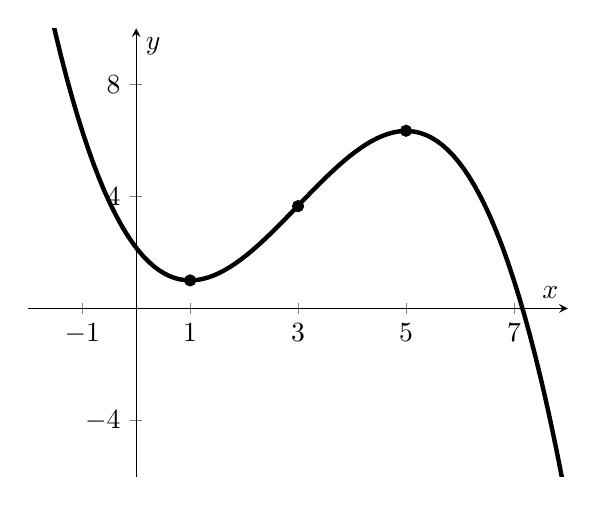
\begin{tikzpicture}
 \begin{axis}[
    xmin = -2, xmax = 8,
    ymin = -6, ymax = 10, xtick={-3,-1,...,7}, ytick={-4, 0,...,8},axis x line=middle, axis y line=
middle, xlabel={$x$}, ylabel={$y$}]
    \addplot[ultra thick, <->,samples=100,
        domain = -2:8,
    ] {1+(x-1)*(x-1)-(1/6)*(x-1)*(x-1)*(x-1)};
    \addplot[mark=*,only marks] coordinates {(1,1)(3,3.65)(5,6.34)};
\end{axis}
\end{tikzpicture}

\columnbreak

\begin{subproblems}
\item $g'(1)$
\item $g''(1)$
\item $g'(3)$
\item $g''(3)$
\item $g'(5)$
\item $g''(5)$
\end{subproblems}
\end{multicols}


\problem{8} Evaluate the limits below. Use algebra to justify your answer. 
	\begin{subproblems}
	\item $\displaystyle \lim_{x \to -\infty} \frac{x^4+1}{x^2-2x^3}$
	\vfill
	\item $\displaystyle \lim_{x \to \infty} \frac{\sqrt{2x^6+x}}{1+x^3} $
	\vfill
	\end{subproblems}
\end{document}

